% !Mode:: "TeX:DE:UTF-8:Main"

\documentclass[aspectratio=169]{beamer}
\usepackage{tikz}
\usetikzlibrary{tikzlings,shadings,decorations.markings}
\usepackage{bearwear}
\usetikzlibrary{decorations.text,fpu}

\setbeamertemplate{navigation symbols}{}

% trick taken from https://topanswers.xyz/tex?q=1989
\tikzset{
    use page relative coordinates/.style={
        shift={(current page.south west)},
        x={(current page.south east)},
        y={(current page.north west)}
    },
}

\makeatletter
\newcommand*{\slideinframe}{\number\beamer@slideinframe}
\makeatother
\setbeamertemplate{background canvas}{}

\tikzset{
  plinth/.pic={
   \path [every edge/.append style={pic actions, opacity=.5}, pic actions]
    (0,0,0) coordinate (o) 
    -- ++(-\cubescale*\cubex,0,0) coordinate (a) 
    -- ++(0,-\cubescale*\cubey,0) coordinate (b) 
    edge[draw=none] 
    ++(0,0,-\cubescale*\cubez)  
    -- ++(\cubescale*\cubex,0,0) coordinate (c) -- cycle;
   \path (o) 
    -- ++(0,0,-\cubescale*\cubez) coordinate (d) 
    -- ++(0,-\cubescale*\cubey,0) coordinate (e) 
    %edge (g) 
    -- (c) -- cycle;
   \fill[gray!50!black] (d) -- (e) -- (c) -- (o) --cycle; 
   \path (o) 
    -- (a) 
    -- ++(0,0,-\cubescale*\cubez) coordinate (f) 
    %edge (g) 
    -- (d) -- cycle;
   \fill[gray!50!white] (o) -- (d) --(f) --(a) --cycle;
 },
  /plinth/.search also={/tikz},
  /plinth/.cd,
  width/.store in=\cubex,
  height/.store in=\cubey,
  depth/.store in=\cubez,
  units/.store in=\cubeunits,
  scale/.store in=\cubescale,
  width=10,
  height=20,
  depth=10,
  units=cm,
  scale=.1,
}

\tikzset{kette/.pic={
 \path[use as bounding box](0,0);
 \begin{scope}[decoration={
markings,% switch on markings
mark=% actually add a mark
between positions 0 and 1 step 0.095
with
{
  \draw[ball color=white] (0,0) circle[radius=1pt];
}
}]
 \draw[white,postaction=decorate](-0.4,1.1)--(0,0.7)--(0.45,1.15);
 \end{scope}
 \fill[ball color=green!90!black] (0,0.7)circle[y radius=5pt,x radius=4pt];
 }
} 

\definecolor{pink}{RGB}{255,20,147}
\begin{document}
\AddToHook{shipout/background} 
   {
    \put(1cm,-4cm){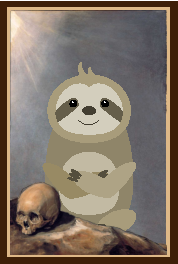
\includegraphics[width=1cm]{ElGreco}}
    \put(4cm,-4cm){
\includegraphics[width=1.5cm]{mondrian}}
    \put(7cm,-4cm){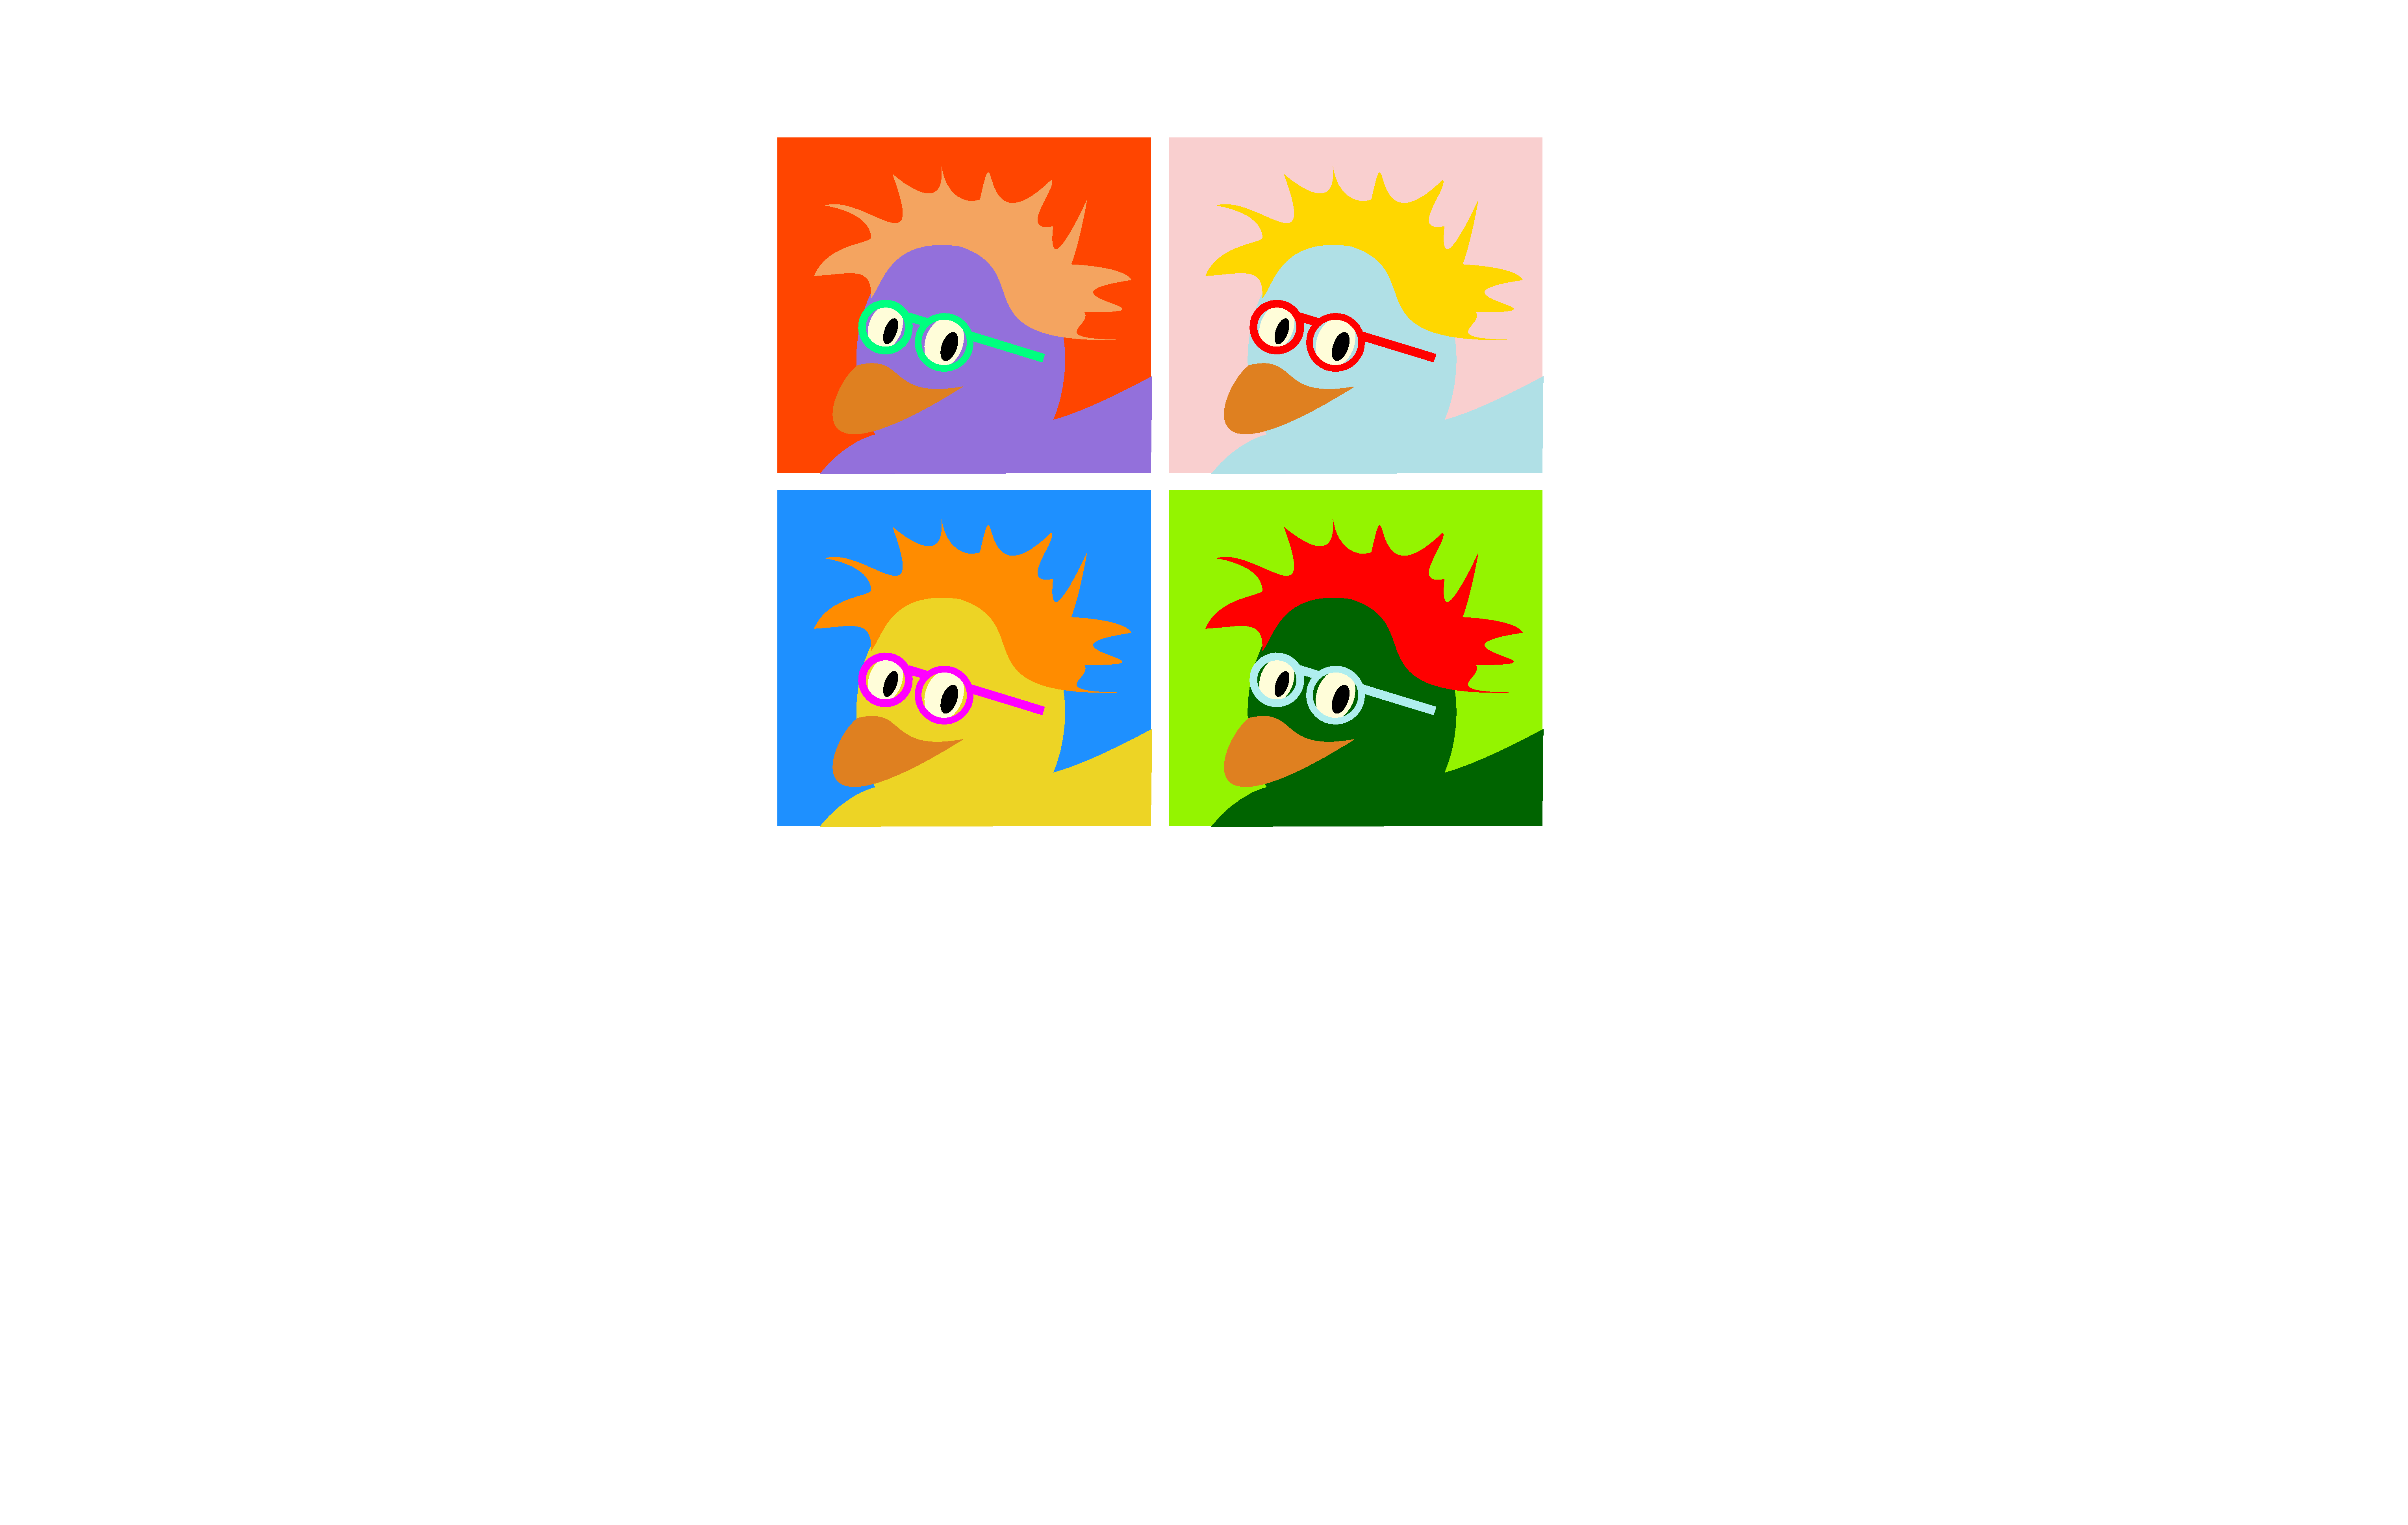
\includegraphics[trim=35cm 29cm 38cm 8cm,width=1.5cm]{PopArt}}
    \put(10cm,-4cm){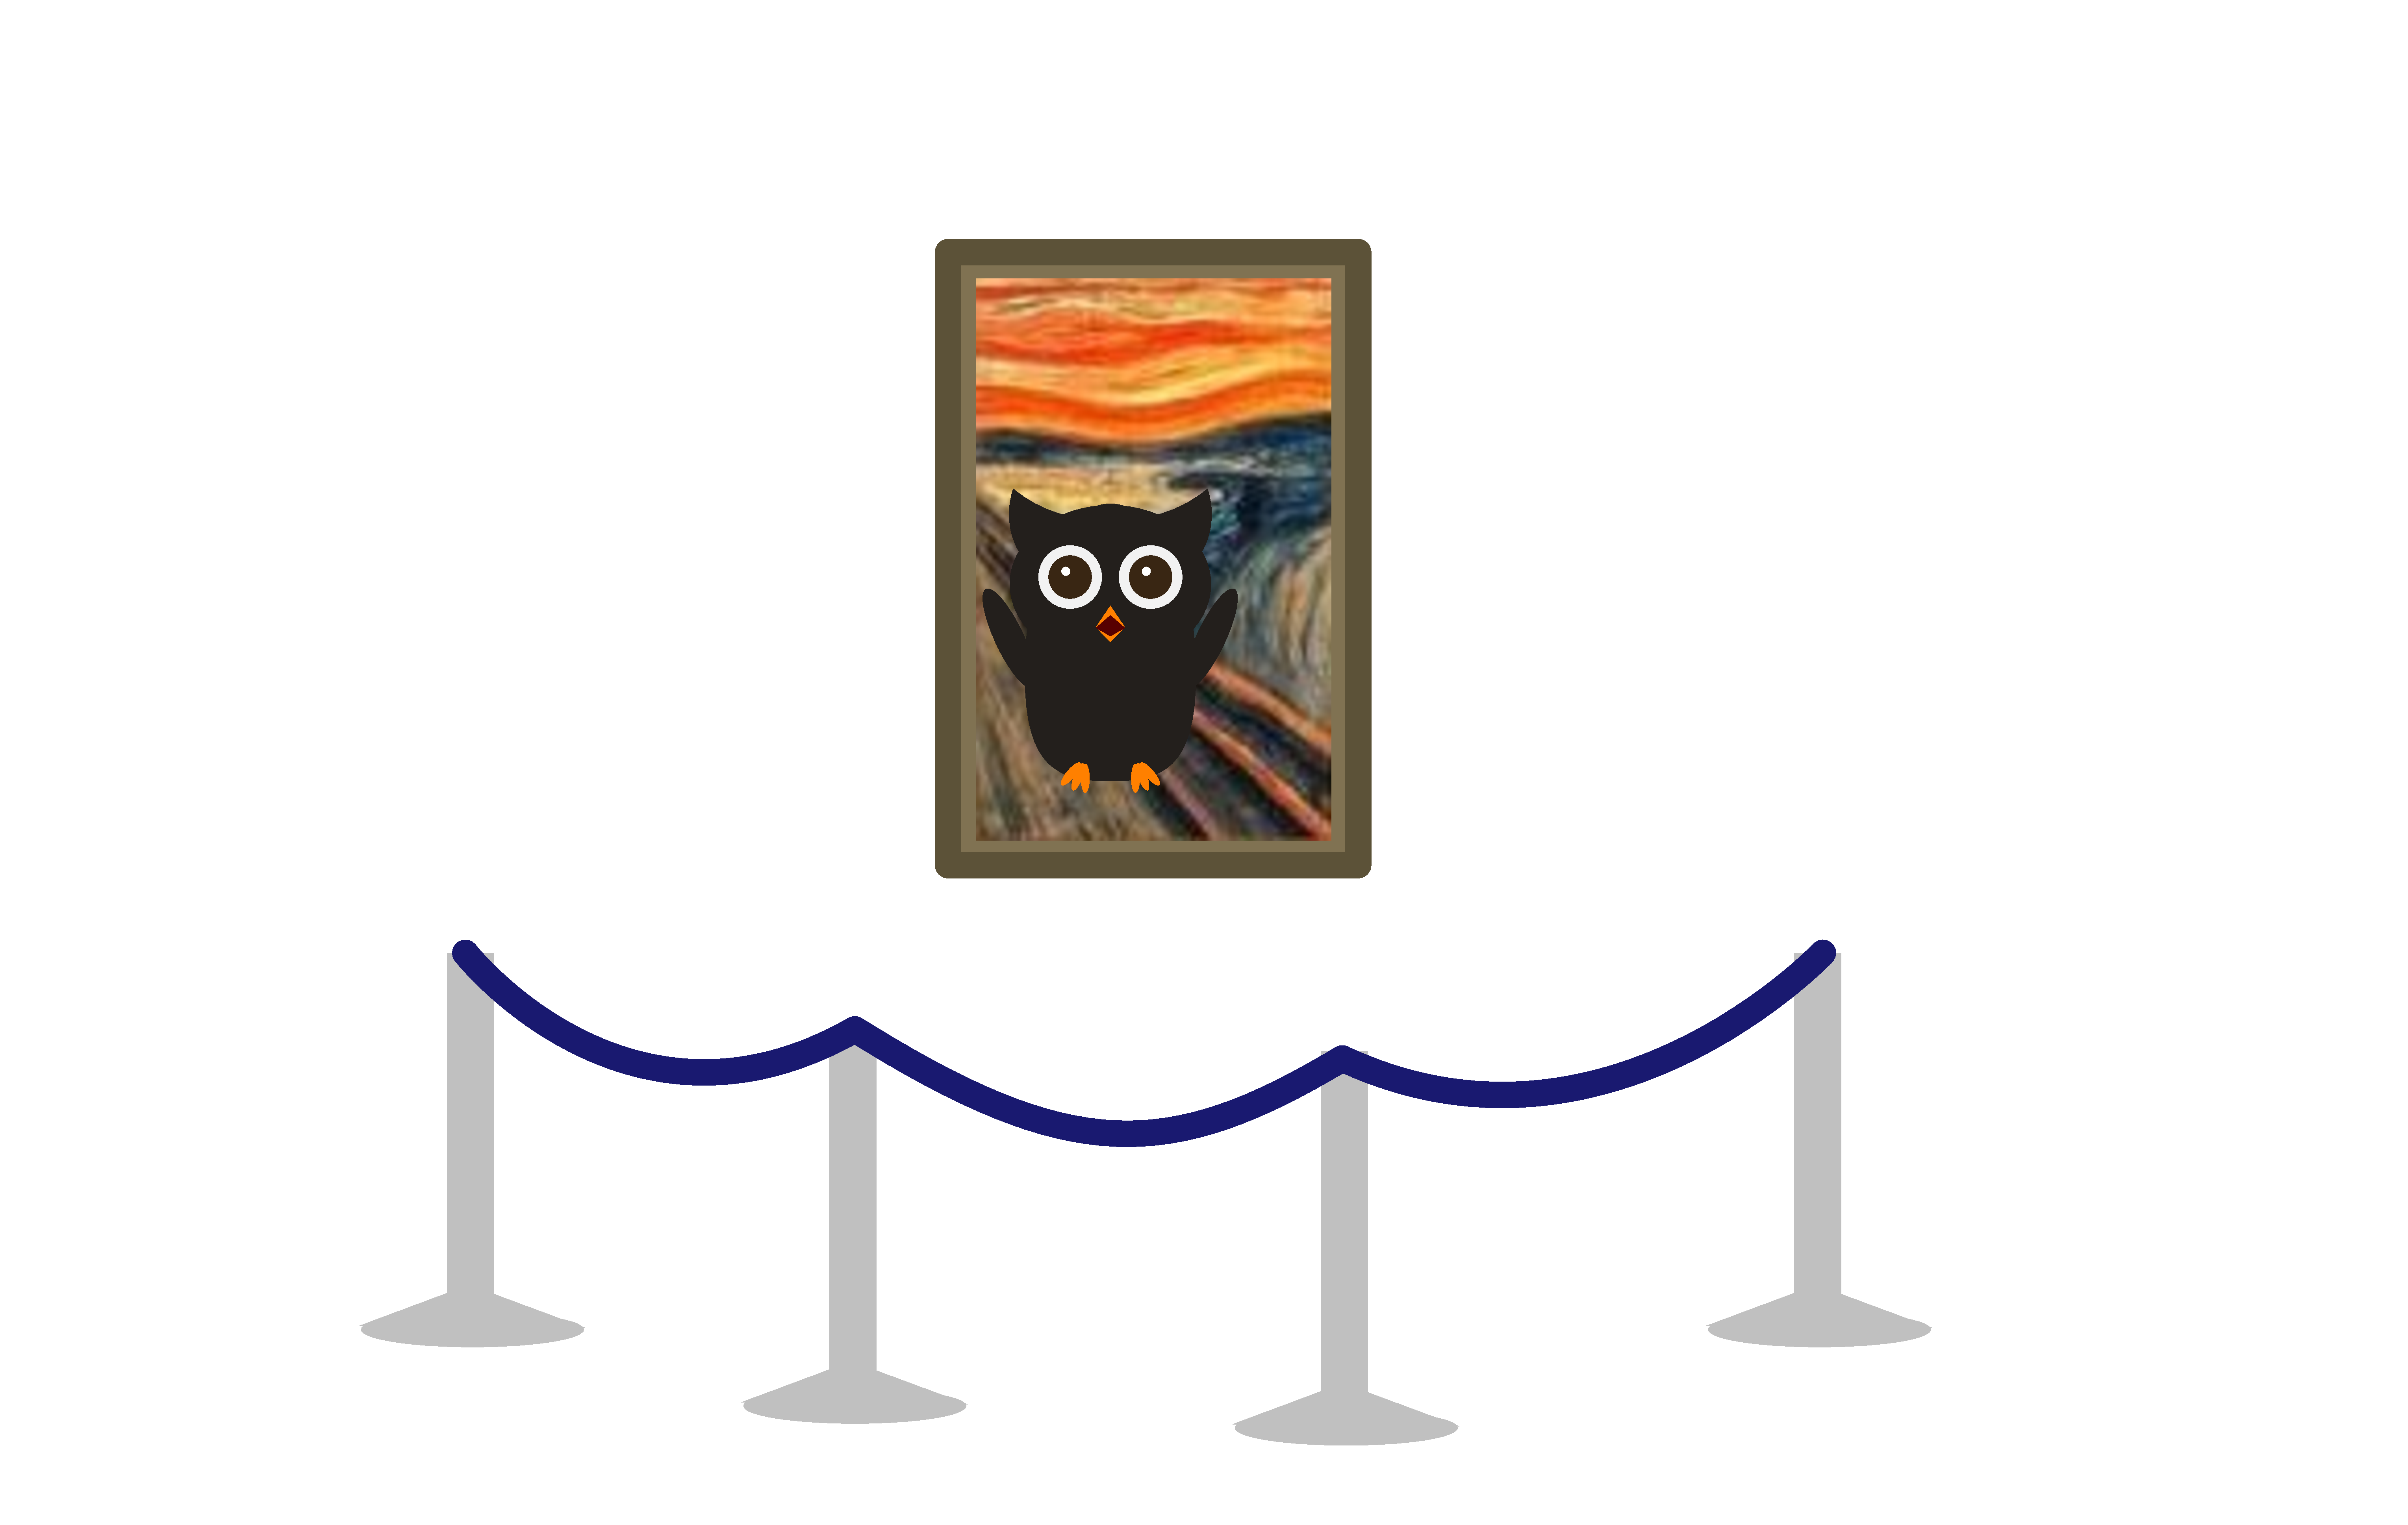
\includegraphics[trim=40cm 29cm 45cm 11cm,width=1cm,clip]{Scream}}
    \put(13cm,-4cm){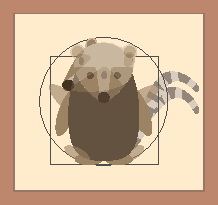
\includegraphics[width=1.5cm]{VitruvianCoati}}
    \put(0,-\paperheight){\textcolor{brown!30!white}{\rule{\paperwidth}{4cm}}}
   } 
\def\steps{350}
\begin{frame}

\vspace{2cm}

\hspace*{2cm}%  
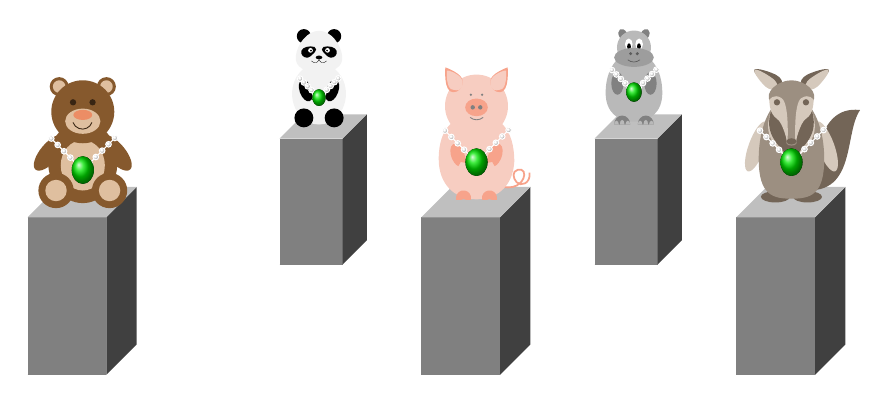
\begin{tikzpicture}[
     %use page relative coordinates,     
  %    remember picture,
  %    overlay
    ]
   
  \path (0,0)pic[fill=gray]{plinth} --++ (-0.3,0.1)pic[scale=0.8]{bear}--++(0,-0.2)pic{kette};
  \path (5,0)pic[fill=gray]{plinth} --++ (-0.3,0.1)pic[scale=0.8]{pig}--++(0,-0.1)pic{kette};
  \path (9,0)pic[fill=gray]{plinth} --++ (-0.3,0.1)pic[scale=0.8]{anteater}--++(0,-0.1)pic{kette};
  \path (3,1)pic[fill=gray,scale=0.8]{plinth} --++ (-0.3,0.1)pic[scale=0.6]{panda}--++(0,0)pic[scale=0.6]{kette};
  \path (7,1)pic[fill=gray,scale=0.8]{plinth} --++ (-0.3,0.1)pic[scale=0.6]{hippo}--++(0,-0)pic[scale=0.7]{kette};
   
  \end{tikzpicture}  
%  \pause[\steps]
 
 
 \end{frame}


\begin{frame}

\vspace{2cm}

\hspace*{2cm}%  
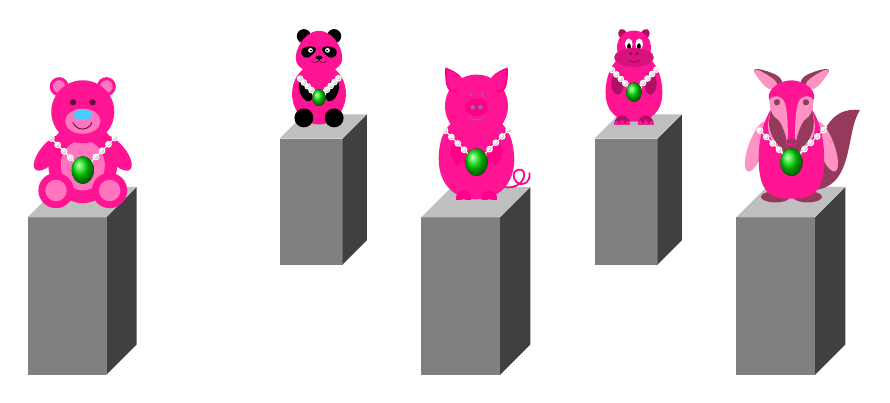
\begin{tikzpicture}[
     %use page relative coordinates,     
  %    remember picture,
  %    overlay
    ]
   
  \path (0,0)pic[fill=gray]{plinth} 
    --++ (-0.3,0.1)pic[bear/body=pink,scale=0.8]{bear}--++(0,-0.2)pic{kette};
  \path (5,0)pic[fill=gray]{plinth} 
    --++ (-0.3,0.1)pic[pig/body=pink,scale=0.8]{pig}--++(0,-0.1)pic{kette};
  \path (9,0)pic[fill=gray]{plinth} 
    --++ (-0.3,0.1)pic[anteater/body=pink,scale=0.8]{anteater}--++(0,-0.1)pic{kette};
  \path (3,1)pic[fill=gray,scale=0.8]{plinth} 
    --++ (-0.3,0.1)pic[panda/body=pink,scale=0.6]{panda}--++(0,0)pic[scale=0.6]{kette};
  \path (7,1)pic[fill=gray,scale=0.8]{plinth} 
    --++ (-0.3,0.1)pic[hippo/body=pink,scale=0.6]{hippo}--++(0,-0)pic[scale=0.7]{kette};
   
  \end{tikzpicture}  
%  \pause[\steps]
 
 
 \end{frame}

\end{document}
